\section{Momentum Resolution}
\label{sec:ep}
 %
To parameterize the smearing due to the momentum resolution the
estimate of the momentum uncertainty provided by the Kalman track fit
is used since it is known to be reliable at the level of $10 \%$ or better.  

%
The LHCb spectrometer is rather complex and consequently the momentum
resolution depends on individual track kinematics. This can be seen in
Fig.  \ref{fig:eppfit} where the calculated uncertainty on the momentum from the
track fit ($\sigma^{fit}_{p}$) divided by $p$ is plotted versus $p$ for tracks from the
combined $\chicone \rightarrow J/\psi \mu^+ \mu^-$ and $\Upsilon(1S) \rightarrow
\mu^+ \mu^-$ samples. Three regions with different performance have been marked with dashed lines:
\begin{description}
\item[IT] These tracks pass through
  the acceptance of the Inner Tracker and consequently benefit from
  its good hit resolution.
\item[OT] These tracks pass through the Outer Tracker which has worse
  hit resolution compared to the Inner Tracker.
\item[High $\eta$] The origin of the worse momentum resolution for this region
  has several causes. Tracks in this region lie at high $\eta$, close to
  the edge of the detector acceptance. They are likely to have no
  information in TT and relatively few VELO hits which worsens the
  resolution. It also seems at least some of these tracks are deflected
  by the magnetic field through the beam-pipe which signficantly worsens their
  momentum resolution since they traverse alot of material
  \footnote{The track sample used contains only muons which are only
    effected by multiple scattering and do not interact hadronically.}. 
\end{description}
%
\begin{figure}[htb!]
\begin{center}
\resizebox{5.0in}{!}{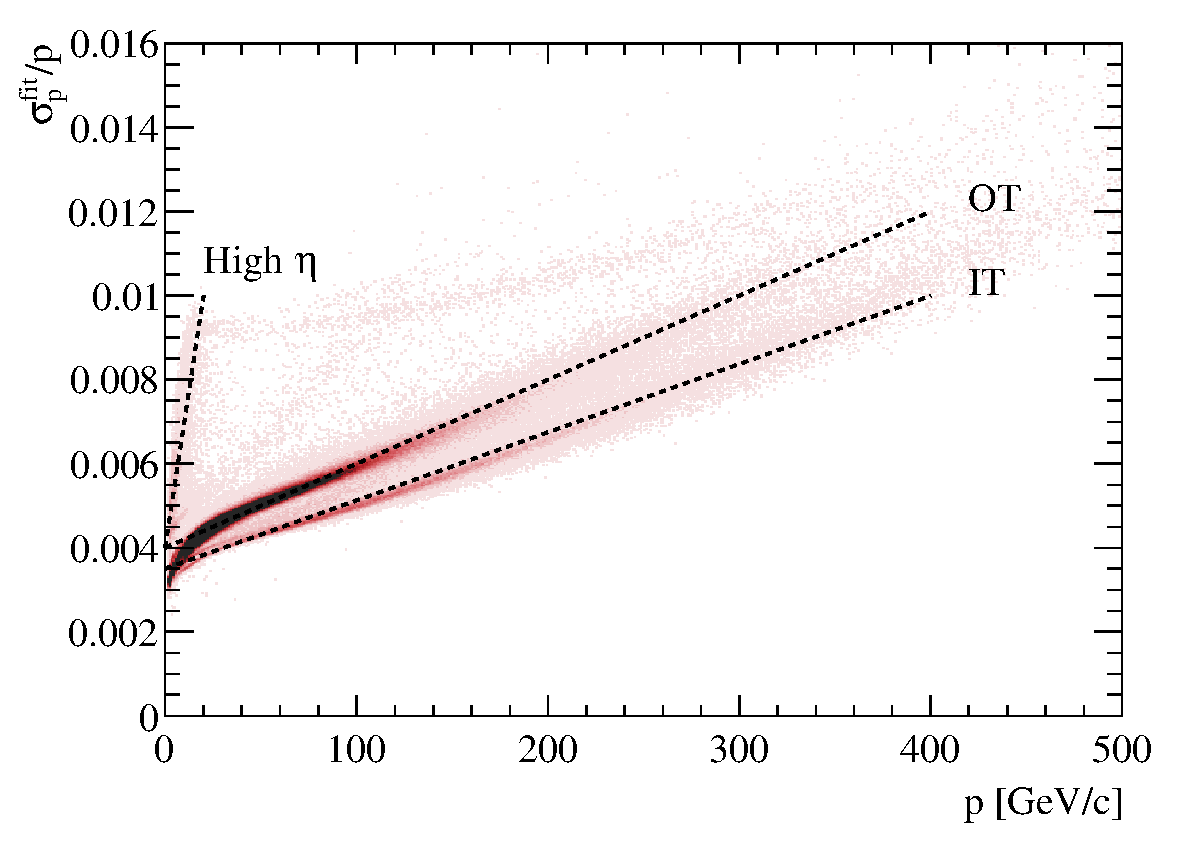
\includegraphics{figs/epp-fit.pdf}}
\caption{\small $\sigma^{fit}_{p}$ versus $p$ for the combined
  $\chicone$ and $\Upsilon$ track sample. }
\label{fig:eppfit}
\end{center}
\end{figure}

For use in a fast simulation these details need to be captured. 
This is a straightforward regression problem with the
input variables being the track kinematics and the target being the
value of $\sigma^{fit}_{P}$ estimated from the track fit. To do this a
Gradient Boosted Decision\footnote{Other methods, e.g. a neural
  network, gave similar results but were more CPU intensive.} tree from the TMVA package \cite{Hocker:2007ht} was
used with the following input variables:
\begin{description}
\item[$\mathbf{p}$] Momentum
\item[$\mathbf{tx}$] Slope in x-direction
\item[$\mathbf{ty}$] Slope in y-direction
\item[$\boldsymbol{\eta}$] pseudorapidity
\item[$\boldsymbol{\phi}$] azimuthal angle
\item[$\mathbf{\pt}$] Transverse momentum
\item[$\mathbf{q\times pol}$] Charge times magnet polarity
%\item[$\mathbf{x_T}$] x position at $9200$ cm 
%\item[$\mathbf{y_T}$] y position at $9200$ cm
\end{description}
The idea of giving both the $(p,tx,ty)$ and $(\pt,\eta,\phi)$
representation is that the detector has some structures (e.g detector
boxes) that are best captured by the first representation and some
(e.g. the 25 mrad cone of the beam-pipe) that are best captured by the
second. 

%The use of the information on the track position in the T-stations
%was found to more accurately capture the high $\eta$ structure in
%Fig. \ref{fig:eppfit}. To calculate $x_T$ and $y_T$ the parameterization
%given in Section~\ref{sec:kick} is used. 
For training the  $\chicone \rightarrow \jpsi \mu^+ \mu^-$ and $\Upsilon(1S) \rightarrow
\mu^+ \mu^-$ samples are used. This allows to cover the full momentum
range of the spectrometer from $3-500 \gevc$ meaning the applicability of this BDT is
wider than the scope of this study. The most highly ranked variables
were $p$, $\eta$ and $\pt$. The performance of the BDT
estimator is good as can be seen from Fig. \ref{fig:corel} and
\ref{fig:diff}. The relative accuracy of the method is $\sim 2.8 \%$
(RMS of Fig. \ref{fig:diff} (Right)) and
it captures the most features of the target distribution well. The
main discrepancy visual is that the long-tail in the high $\eta$ region is
not well reproduced. 
%
\begin{figure}[h!]
\centering
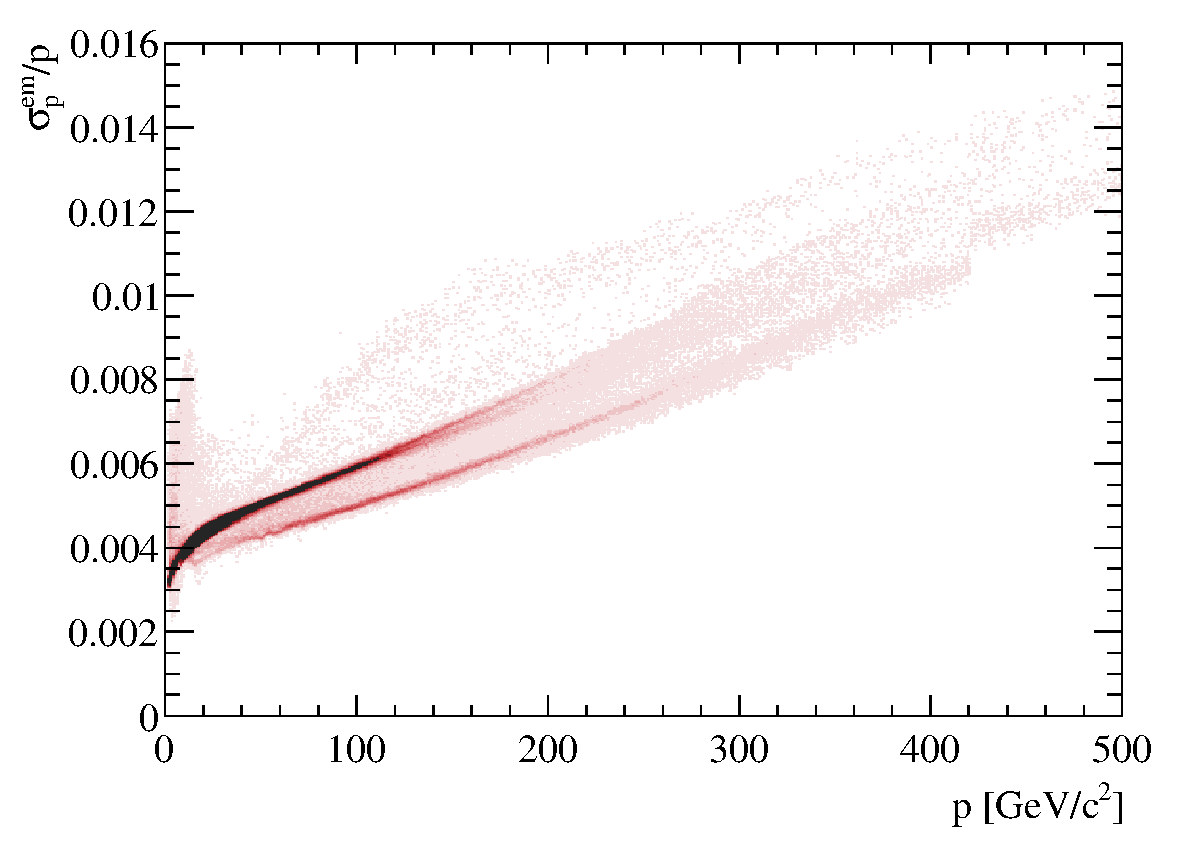
\includegraphics[width=0.48\textwidth]{figs/epp-em.pdf}
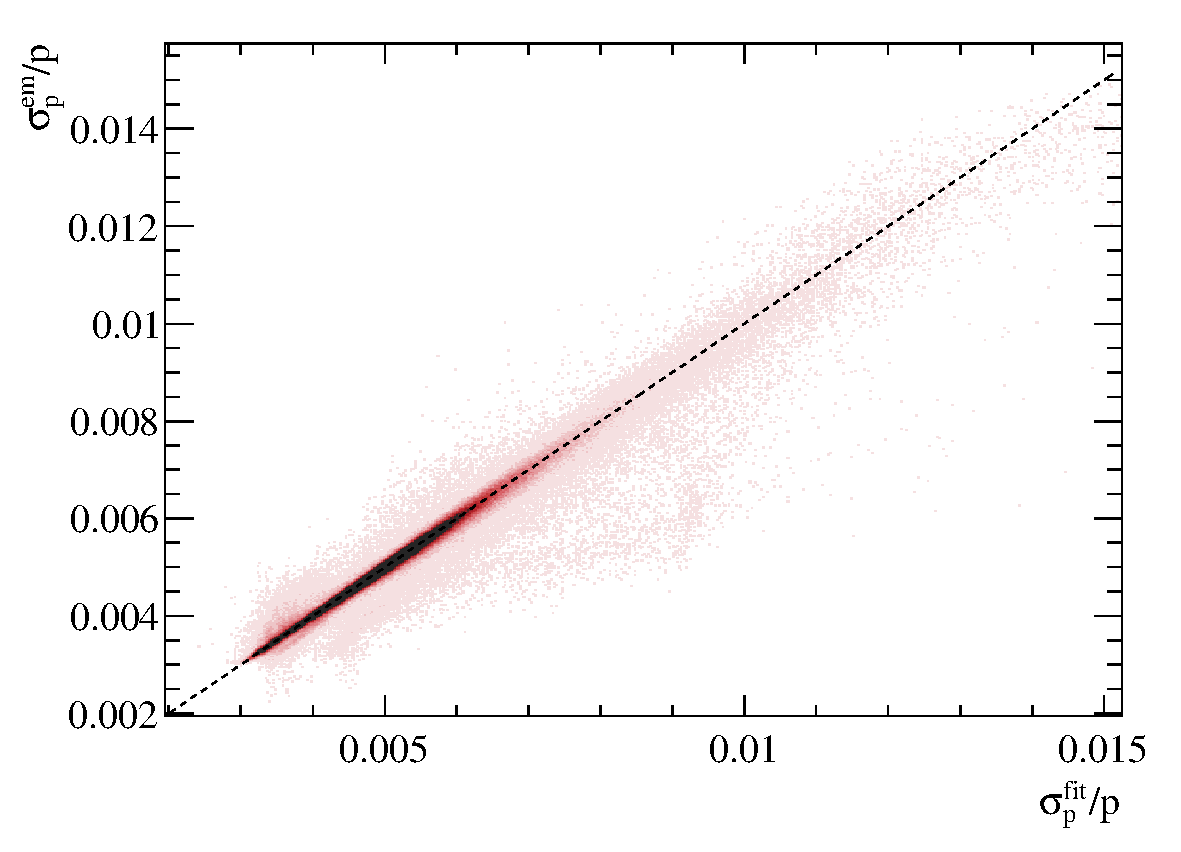
\includegraphics[width=0.48\textwidth]{figs/corelation.pdf}
\caption{(Left) $\sigma^{em}_{p}$ versus $p$ and (Right)
  $\sigma^{em}_{p}$  versus  $\sigma^{fit}_{p}$. The dotted line
  corresponds to perfect corelation. Both plots are made with the combined
  $\chicone$ and $\Upsilon$ sample.  }
\label{fig:corel}
\end{figure}
%
\begin{figure}[h!]
\centering
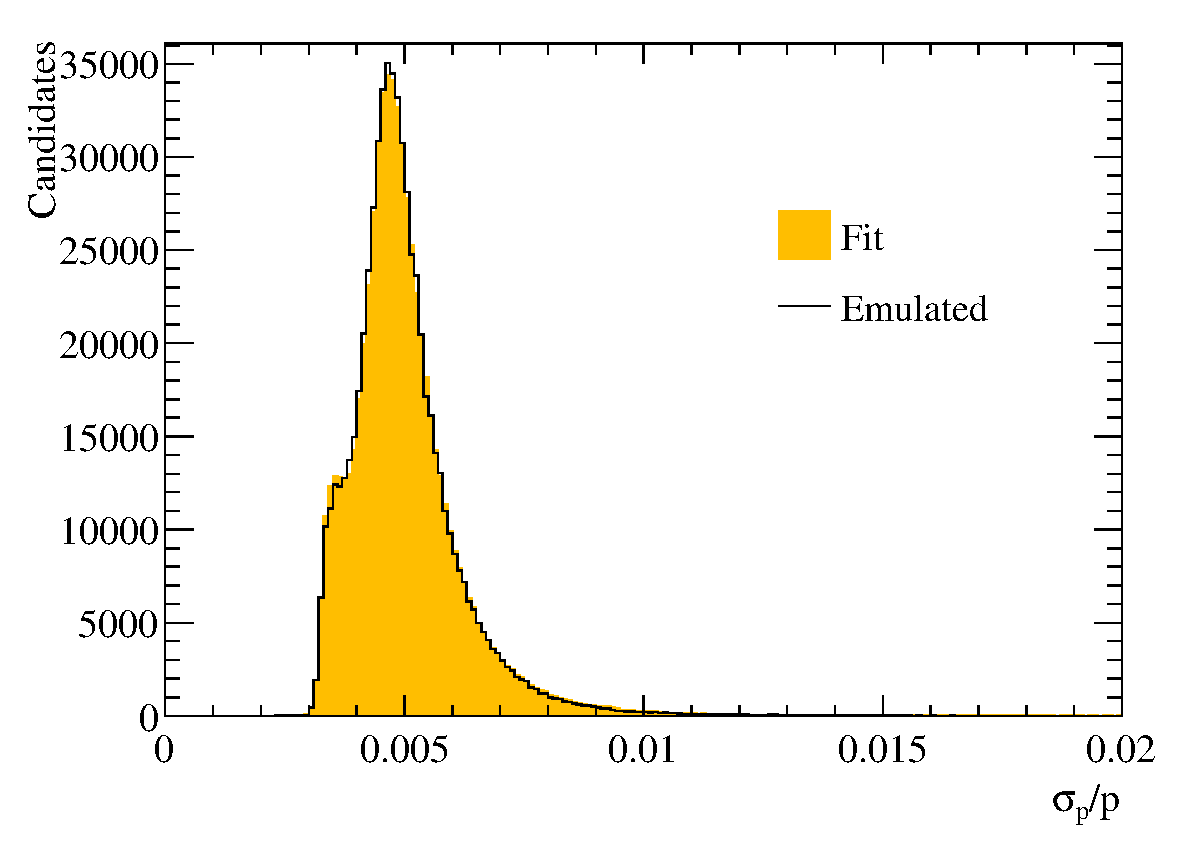
\includegraphics[width=0.48\textwidth]{figs/ep.pdf}
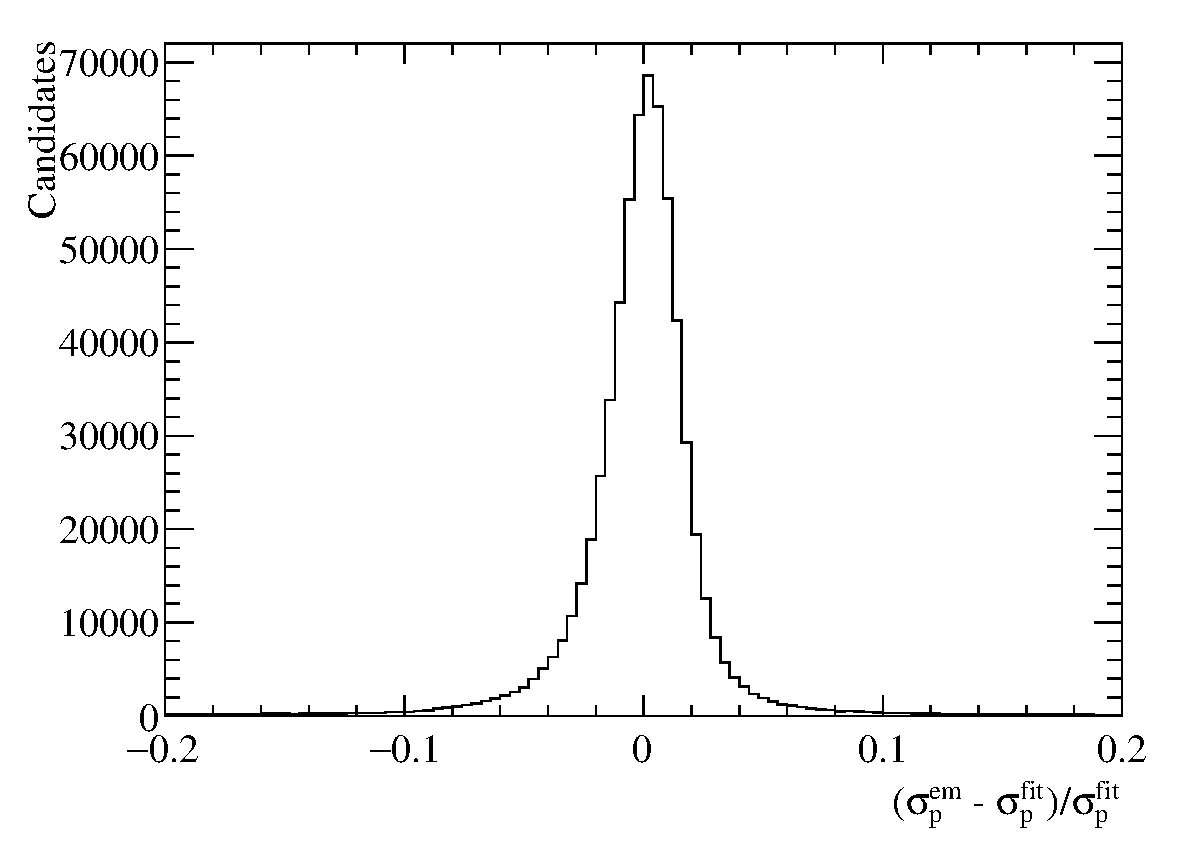
\includegraphics[width=0.48\textwidth]{figs/difference.pdf}
\caption{(Left) Distribution of $\sigma^{em}_{p}$ and
  $\sigma^{fit}_{p}$. The shape of this distribution reflects the
  input samples used for training. (Right) Distribution of the relative difference between $\sigma^{em}_{p}$ and
  $\sigma^{fit}_{p}$  }.
\label{fig:diff}
\end{figure}

The quality of this estimate can be judged from the pull, defined as 
\begin{equation*}
\frac{p_{rec} - p_{true}}{\sigma^{em}_{p}}.
\end{equation*}
Figure \ref{fig:ppull} shows the resulting pull distribution. The RMS of this
distribution is 1.2. The tails are expected and due to the fact that there are
non-Gaussian tails in the energy loss and multiple scattering
processes that are not captured by the Kalman filter. Fitting a double
Gaussian gives a central core with a width 0.93 and a wider Gaussian
with width 1.9. The fraction in the core is $92 \%$. It is easy to
incoporate these values into the emulator by using double Gaussian
smearing.  The pull distribution
also exhibits a small bias (0.09), probably due to the tail in the energy loss
distribution. This bias is ignored for the emulation \footnote{The
  momentum scale in the full simulation is known to need tuning. For
  the use case envisaged of $\chi_{b}$ Dalitz decays the momentum
  scale on data is readily cross-checked with other modes.}.
%
\begin{figure}[htb!]
\begin{center}
\resizebox{3.8in}{!}{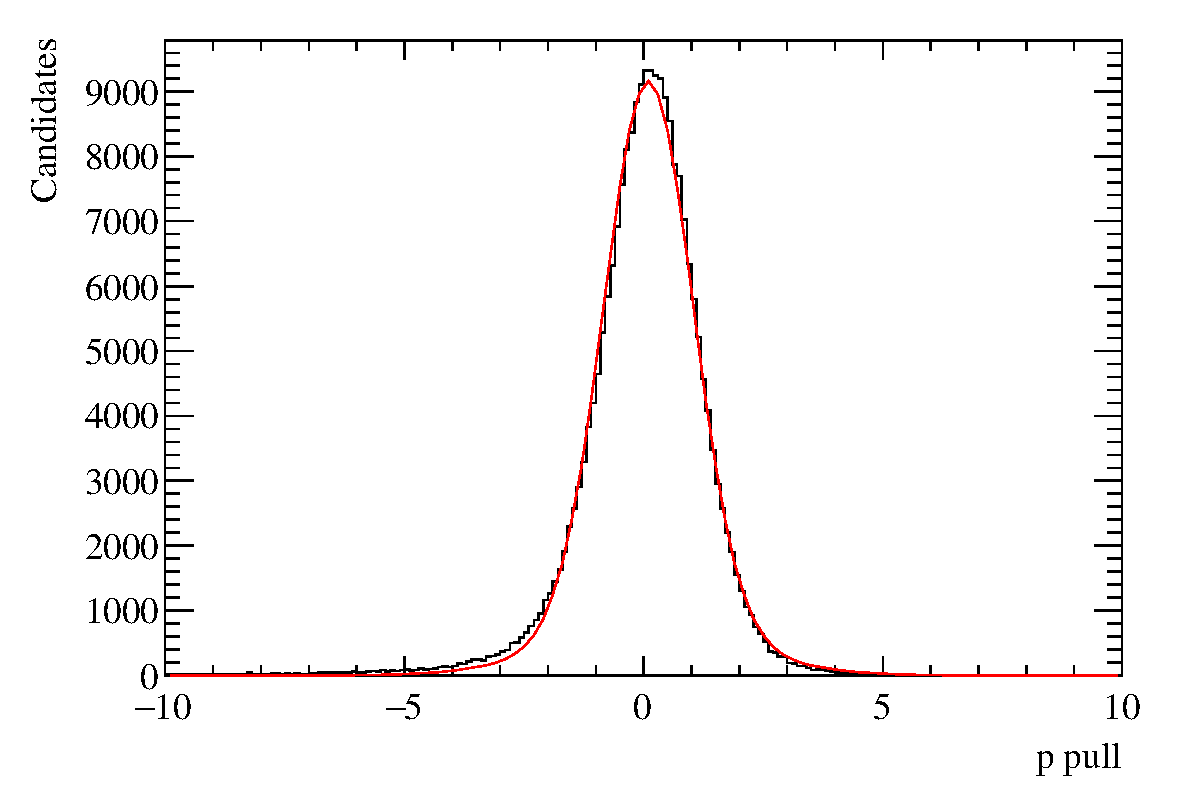
\includegraphics{figs/pullp.pdf}}
\caption{\small Momentum pull using the emulation. A fit to a double
  Gaussian function is superimposed.}
\label{fig:ppull}
\end{center}
\end{figure}
